\emph{Artificial neural networks} or simply \emph{neural networks} are one of the most popular nonlinear classifiers used today. They were initially inspired by the way biological neurons process information coming from its dendrites and relaying it through its axon to neighboring neurons~\cite{McCulloch1943, Widrow1960, Rosenblatt1962} but evolved to become more practical for nonlinear modelling albeit less biologically accurate~\cite{Rumelhart1986}. We discuss here multilayer feedforward neural networks, the name should become obvious after a few paragraphs.

\emph{Multilayer feedforward neural networks} are composed of $L$ layers of \emph{neurons}, units of computation, each of which is fully connected to the next and previous layer (except for the first and last layer). The first layer, called the \emph{input layer}, has $s^{(1)} = n$ units and receives the feature vector $x \in \mathbb{R}^n$ meanwhile the last layer or \emph{output layer} has $s^{(L)} = K$ units corresponding to the $K$ possible classes. Every other layer is called a \emph{hidden layer} (see Fig.~\ref{fig:NeuralNetwork} for an example). The neural network receives an input $x \in \mathbb{R}^n$, processes it layer by layer and outputs a vector $h_\Theta(x) \in \mathbb{R}^K$, where $h_\Theta(x)_k$ is the predicted (unnormalized log) probability that $x$ belongs to class $k$. Each unit performs a computation on the input from the units in the previous layer and transmits the result to the units in the next layer through its connections. Furthermore, each connection has a \emph{weight} $w$ which is to be learned in the training phase, i.e, the weights are the parameters $\Theta$ of the model. A neural network is said to be \emph{shallow} or \emph{deep} according to its number of layers or \emph{depth}.\footnote{There is no consensus on when a neural network becomes a deep neural network\cite{Schmidhuber2015}. We consider networks with over 2 hidden layers to be deep.}

\begin{figure}[h]
	\centering
	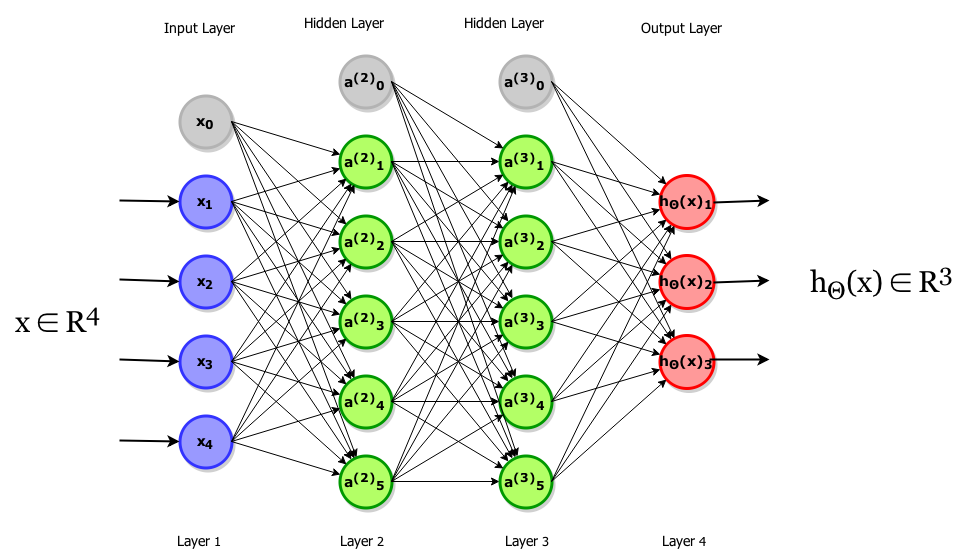
\includegraphics[width = \textwidth]{plots/neuralNetwork.png}
	\caption[Example of an Artificial Neural Network]{Small neural network example. Input layer with 4 units (blue), two hidden layers of 5 units (green) and output layer of 3 units(red). Bias units appear in gray. It approximates a function $h_\Theta(x): \mathbb{R}^4 \to \mathbb{R}^3$, i.e., it classifies an input vector $x \in \mathbb{R}^4$ into 3 possible classes.}
	\label{fig:NeuralNetwork}
\end{figure}

A unit $i$ in layer $l$ computes a function of the form:
\begin{equation}
	a^{(l)}_i = g \left(\sum_{j=0}^{s^{(l-1)}} \Theta^{(l-1)}_{ij}a_j^{(l-1)}\right) \text{ for $l= 2,\dots,L-1$ and $i = 1,\dots,s^{(l)}$}
	\label{eq:NeuronActivation}
\end{equation}
where $a^{(l)}_i$ is called the \emph{activation} or output of unit $i$ in layer $l$;
$g(\cdot)$ is an \emph{activation function} (defined below);
$s^{(l)}$ is the number of units in layer $l$;
$a^{(u)}_0 = 1$, for all $u = 1, \ldots, L-1$ (bias units);
$a^{(1)}_v = x_v$ for all $v = 1, \ldots, n$ i.e, the activation of the input layer is the input $x$;
$a^{(L)}_i = \sum_{j=0}^{s^{(L-1)}} \Theta^{(L-1)}_{ij}a_j^{(L-1)}$ for all $i = 1,\dots,s^{(L)}$ i.e, $g(\cdot)$ is not applied in the output layer
and $\Theta^{(l)} \in \mathbb{R}^{s^{l+1} \times s^{l}} $ is the matrix of weights connecting layer $l$ to $l+1$. At each layer (except the output layer) we include a unit which always emits activation 1 ($a^{(1)}_0 = 1$, $a^{(2)}_0 = 1$, etc), these are called \emph{bias units}~
\footnote{They are included for a technical detail: so that the activation function $g(w^Tx+w_0)$ can shift in the x-axis changing its threshold to $-w_0$, which is learned by the neural network.}. 
The bias units are assumed to be included into each vector $a^{(l)}$, hence the sumation in Equation~\ref{eq:NeuronActivation} starts at 0 and not 1. It may seem like a convoluted definition but it simply defines the activation of a given unit as the weighted linear combination of activations of the units in the previous layer passed through a nonlinear function $g(\cdot)$.
Lastly, notice that $a^{(L)} \in \mathbb{R}^{s^{(L)}}$, the vector of activations in the last layer of the network, is equal to the predicted (unnormalized log) probabilities $h_\Theta(x) \in \mathbb{R}^K$, also called a \emph{score vector}. The class with the highest score in $h_\Theta(x)$ is the predicted class for the example $x$. We could also exponentiate each of these probabilities and normalize them to obtain a distribution of probabilities over the possible classes $K$ ($p(x) \in [0..1]^K$). This improves interpretability but does not change the predicted classes.

\begin{comment}
The activation function $g(\cdot)$ is usually a \emph{logistic sigmoid function}:
\begin{equation}
	g(z) = \frac{1}{1+ e^{-z}}
\end{equation}
The sigmoid function has range [0,1] and is differentiable with respect to $z$. Because of this characteristics it is used to represent probabilities in the logistic regression classifier. \emph{Logistic regression} for binary classification models the probability that $x \in \mathbb{R}^n$ belongs to the positive class as $g(w^Tx)$ and estimates the parameters $w \in \mathbb{R}^n$ during training. Any input whose output $g(w^Tx)$ is greater than $0.5$ is classified as positive, otherwise it is classified as negative. The sigmoid function equals $0.5$ when $w^Tx = 0$, thus, the decision boundary of a logistic regression classifier is $w^Tx = 0$, which is a linear function. 

However, the sigmoid function, per se, is not linear on its input $z$. Therefore, each unit in a neural network with sigmoid activation functions outputs a nonlinear activation $g(z)$ which in turn is received by units in the next layer, linearly recombined with the activation of other units and passed again through a sigmoid function; these operations are repeated until the input reaches the output layer. As a result, the function calculated by units in the output layer $h_\Theta(x)$ will be highly nonlinear on the original input $x$. This is the reason why neural networks can model functions which are highly nonlinear and why increasing the number of layers in a neural network increases the predictive power of the model. By the same token, it may be insightful to think of each unit in a neural network as a feature detector (via logistic regression): units in the first hidden layer are trained to activate when simple features are found on the input, units on the second hidden layer activate when a combination of these simple features is present on the input and so on. Thus, the network will learn to detect the most relevant features for the classification task and as the number of units increases, it learns ever more complex features (granted that there is enough training data).
\end{comment}

The activation function $g(\cdot)$ is usually a \emph{rectified linear unit} or \emph{ReLU}:
\begin{equation}
	g(z) = \max(0,z)
\end{equation}
This is a nonlinear activation function which is very easy to implement in numerical computations, its derivative ($1_{z>0}$) can be calculated quickly and does not suffer from vanishing or exploding gradients as do the sigmoid or tanh activation functions. Furthermore, it has been shown to greatly accelerate the convergence of gradient descent~\cite{Krizhevsky2012}. For these reasons it is the currently recommended activation function for deep neural networks~\cite{Karpathy2015}.

Each unit in a neural network outputs a nonlinear activation $g(z)$ which in turn is received by units in the next layer, linearly recombined with the activation of other units and passed again through a nonlinear function; these operations are repeated until the input reaches the output layer. As a result, the function calculated by units in the output layer $h_\Theta(x)$ will be highly nonlinear on the original input $x$. This is the reason why neural networks can model functions which are highly nonlinear and why increasing the number of layers in a neural network increases the predictive power of the model. By the same token, it may be insightful to think of each unit in a neural network as a feature detector: units in the first hidden layer are trained to activate when simple features are found on the input, units on the second hidden layer activate when a combination of those simple features is present on the input and so on. Thus, the network will learn to detect the most relevant features for the classification task and as the number of units increases, it learns ever more complex features (as long as there is enough training data).

The \emph{softmax} cost function for a multiclass neural network classifier is defined as:
\begin{equation}
	J(\Theta) = -\frac{1}{m} \sum_{i=1}^m \log \left ( \frac{ e^{h_\Theta(x^{(i)})_{y^{(i)}}} }{ \sum_{j=1}^K e^{ h_\Theta (x^{(i)})_j} } \right )
\end{equation}
where $m$ is the number of examples in the training set, $h_\Theta(x)$ is the score vector, $K$ is the number of classes and $(x^{(i)},y^{(i)})$ is the $i^{th}$ example. $J(\Theta)$ is differentiable with respect to $\Theta$ but non-convex, nonetheless, gradient descent usually converges to a good estimate of the network weights~\cite{Ng2014}. \emph{Error backpropagation}~\cite{Linnainmaa1970, Werbos1974}, an algorithm to calculate the derivatives with respect to $\Theta$ needed for gradient descent, computes the error terms in the output layer and backpropagates them layer by layer using the chain rule of derivatives. Given the big number of parameters which need to be estimated, neural networks are susceptible to overfitting. The simplest approach to overcome this problenm is to use regularization. Regularization for neural networks is done by performing gradient descent on the regularized cost function presented in Equation~\ref{eq:ANNRegularizedCostFunction}
\begin{equation}
	J(\Theta) = -\frac{1}{m} \sum_{i=1}^m \log \left ( \frac{ e^{h_\Theta(x^{(i)})_{y^{(i)}}} }{ \sum_{j=1}^K e^{ h_\Theta (x^{(i)})_j} } \right ) + \frac{\lambda}{2m}\sum_{l=1}^{L-1}\sum_{i=1}^{s^{(l)}}\sum_{j=1}^{s^{(l+1)}} \left(\Theta^{(l)}_{ij}\right)^2
	\label{eq:ANNRegularizedCostFunction}
\end{equation}
